\clearpage
\section{Methods}
\label{sec.methods}

% In order to have a quantitative definition of information, three approaches are known: combinatorial, probabilistic and algorithmic~\cite{kolmogorov1965three}, of which probabilistic and algorithmic ones are more popular. By the algorithmic approach, which is followed up by, e.g., Zenil \textit{et~al} in~\cite{zenil2018decomposition,zenil2018algorithmic,soler2017computable}, algorithmic complexity can be approximated based upon the theory of algorithmic probability, namely by the coding theorem method (CTM) and block decomposition method (BDM). In this paper, we follow a combination of probabilistic and algorithmic approaches, although it has a closer connection to the probabilistic one. The proposed amino acid compression method, AC, is based upon a cooperation between finite-context models (FCMs)~\cite{pinho2011representability,pinho2013mfcompress} and substitutional tolerant Markov models (STMMs)~\cite{pratas2016efficient,pratas2017substitutional}. The FCMs follow the probabilistic approach by computing the probability of the next symbol in a sequence, considering the $k$ most recent symbols. This is while the STMMs tend to follow the algorithmic approach by being enabled/disabled based on their performance. It is worth mentioning that the proposed method has been partially published in~\cite{pratas2018compression}. The current paper provides an extensive description of the method along with the results of additional and brand-new experiments. 

% In the following sections, we describe the AC method in great detail. Then, we compare the results of running AC and other compressors on a collection of sequences from several domains and kingdoms. Finally, we present an analysis based on the results of carrying out our compressor on a large collection of reference proteomes.


% % \section{Method} \label{meth}
% AC is based on cooperation between finite-context models and substitutional tolerant Markov models with several depths. The mixture weights associated with each model are updated based on its performance, which is related to the specific forgetting function of each model.


% \subsection{Finite-context models} \label{fcm}
% A finite-context model, relying on the Markov property, considers the $k$ most recent symbols  of an information source (context size of $k$) in order to estimate the probability of the next symbol~\cite{sayood2017introduction,pinho2011representability,pinho2013mfcompress}. Denoting the $k$ most recent symbols as $x_{i-k}^{i-1} = x_{i-k} x_{i-k+1}\cdots x_{i-1}$, the probability of the next symbol $s$, in the position $i$, is estimated as
% \begin{equation} \label{eq:estimate}
% P_m(s|x_{i-k}^{i-1}) = \frac{N(s|x_{i-k}^{i-1})+\alpha}{N(x_{i-k}^{i-1})+ \alpha|\Theta|},
% \end{equation}
% in which $m$ denotes the context model, $N(s|x_{i-k}^{i-1})$ represents the number of times that the information source has generated symbol $s$ in the past, $\Theta$ is the alphabet and $N(x_{i-k}^{i-1}) = \sum_{j \in \Theta} N(j|x_{i-k}^{i-1})$ denotes the total number of events occurred associated with the context~$x_{i-k}^{i-1}$. The parameter $\alpha$ allows balancing between the maximum likelihood estimator and a uniform distribution. Note, for large number of events $i$, the estimator behaves as a maximum likelihood estimator. Also, for $\alpha=1$, Eq.~\ref{eq:estimate} turns to the Laplace estimator~\cite{pratas2015alignment}.

% \subsection{Substitutional tolerant Markov models} \label{stmm}
% A substitutional tolerant Markov model (STMM) \cite{pratas2016efficient,pratas2017substitutional} is a probabilistic-algorithmic context model. 
% An\linebreak STMM uses the occurrence probabilities stored in the memory and assumes that the symbol to be seen in the sequence is the one with the highest probability. This way, it does not take into consideration the symbol that actually is in the sequence. 

% Considering the $k$ most recent symbols, the probability of the next symbol $s$ is estimated as
% \begin{equation}
% P_m(s|{x'}_{i-k}^{i-1}) = \frac{N(s|{x'}_{i-k}^{i-1})+\alpha}
% {N({x'}_{i-k}^{i-1})+ \alpha|\Theta|},
% \end{equation}
% in which $N$ is the memory counts regarding the model and $x'$ is a copy of the context $x$ that is modified as 
% \begin{equation}
% {x'}_{i} = \argmax_{\forall s \in \Theta}{P_m(s|{x'}_{i-k}^{i-1})}.
% \end{equation}

% An STMM is an algorithmic model, namely because it can be disabled and enabled based on its performance. This operation is done considering a predefined threshold $t$. For this purpose, a cache array (history) with the size of $k$ (context-order size) is used to store the recent $k$ hits/misses. When we see a symbol in the sequence, if it is the most probable symbol, based on the number of occurrences saved in the memory, a hit will be stored in the history array; otherwise, a miss will be stored. At the time of seeing a symbol, before storing any hit/miss in the history, we check the number of misses. If it is greater than the threshold $t$, the STMM will be disabled and the history will be reset. This process starts over again for the next symbol.

% To make the difference of FCM and STMM clearer, we give an example. Assume, the current context is\linebreak $c_0=\textrm{FDCAE}$, with $k=5$, and the number of occurrences stored in the memory are $\textrm{F}=8$, $\textrm{D}=5$, $\textrm{C}=12$, $\textrm{A}=7$ and $\textrm{E}=10$. Also, assume the next symbol in the sequence, which is to be compressed, is $\textrm{A}$. Based on an FCM, the next context will be $c_1=\textrm{DCAEA}$, while based on an STMM, it will be $c'_1=\textrm{DCAEC}$. This is because an FCM considers the next symbol as the actual one seen in the sequence, i.e. $\textrm{A}$, but an STMM considers it as the most probable symbol, $\textrm{C}$. This way, the STMM assumes the next symbol to be compressed is $\textrm{C}$, instead of $\textrm{A}$.

% \subsection{Cooperation of FCMs and STMMs} \label{cooper}
% In the case of cooperation between FCMs and STMMs, considering the $k$ most recent symbols in the sequence, the probability of the next symbol $s$ is estimated as
% \begin{equation}
% P(s) = \sum_{m\in\mathcal{F}} P_m(s|x_{i-k}^{i-1})\;w_{m,\,i} + \sum_{m\in\mathcal{S}} P_m(s|{x'}_{i-k}^{i-1})\;w_{m,\,i},
% \end{equation}
% where $\mathcal{F}$ is the set of FCMs and $\mathcal{S}$ is the set of STMMs. $P_m(s|x_{i-k}^{i-1})$ and $P_m(s|{x'}_{i-k}^{i-1})$ are the probabilities of the next symbol estimated by the FCM and the STMM, respectively. Also, $w_{m,i}$ is a weight assigned to each model, based on its performance. For this weighting factor, we have
% \begin{align}
% &\forall m\in\mathcal{F}:\quad w_{m,i} \propto (w_{m,i-1})^{\gamma_m} P_m(s | x_{i-k-1}^{i-2})
% \nonumber
% \\[1mm]
% &\forall m\in\mathcal{S}:\quad w_{m,i} \propto (w_{m,i-1})^{\gamma_m} P_m(s | {x'}_{i-k-1}^{i-2}),
% \end{align}
% in which $\gamma_m \in [0,1)$ acts as a forgetting factor for the models. Note,
% \begin{equation}
% \sum_{m\in\mathcal{F}} w_{m,i} + \sum_{m\in\mathcal{S}} w_{m,i} = 1.
% \end{equation}
% We have found that the lower the context-order size $k$, the lower $\gamma_m$ should be assigned to the model, and vice~versa. For example, for a model with $k=6$, a $\gamma_m \simeq 0.9$ and for a model with $k=18$, a $\gamma_m \simeq 0.95$ is the appropriate choice. This means, the more complex the model, the less the forgetting intensity.

The schema of the proposed method is illustrated in Fig.~\ref{fig.schema}. \smashpp takes as inputs a reference and a target file and produces as output a position file, which is then fed to the \smashpp visualizer to produce an SVG image. This process has eight major stages: (1)~compression of the original target file, based on the model of original reference file, (2)~filtering and segmentation of the compressed file, (3)~reference-free compression of the segmented files, obtained by the previous stage, (4)~compression of the original reference file, based on the model of segmented files obtained by stage~2, (5)~filtering and segmentation of the compressed files, (6)~reference-free compression of the segmented files, that are obtained by the stage~5, (7)~aggregating positions, generated by stages~3 and~6, and (8)~visualizing the positions. The following sections describe the process in detail.

\begin{figure}[!h]
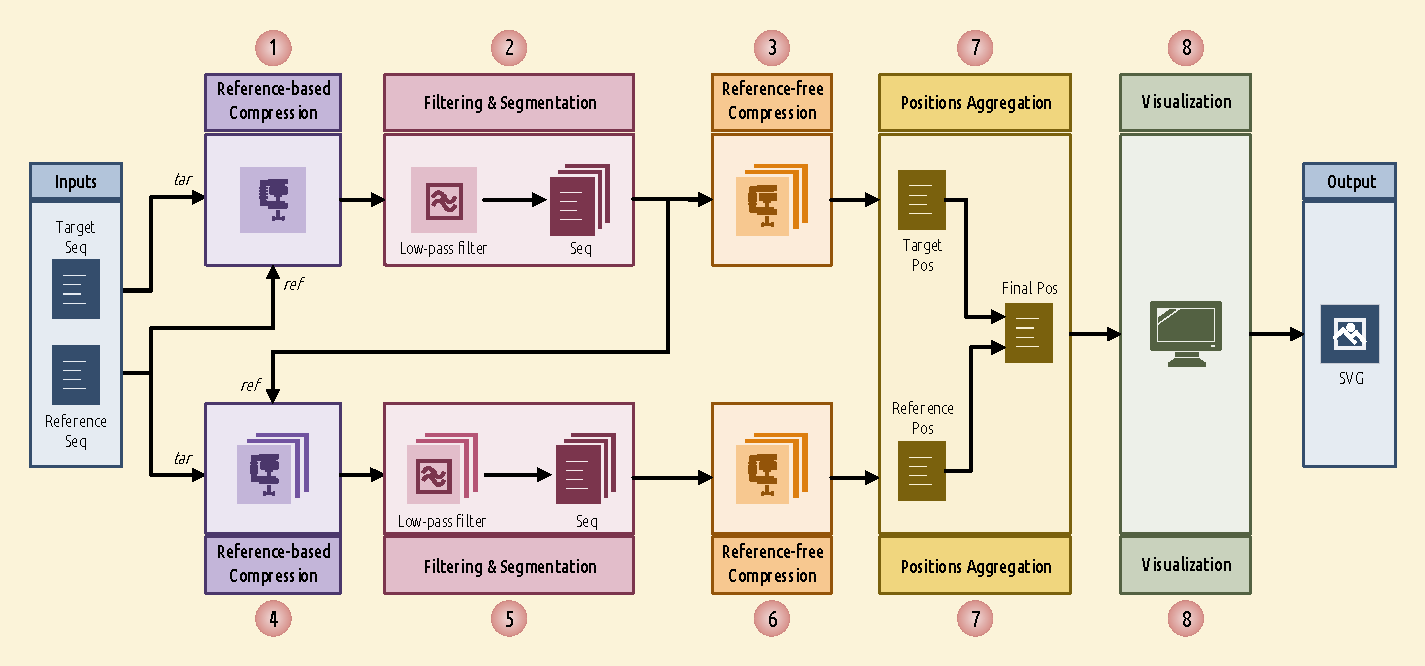
\includegraphics[width=\linewidth]{schema.pdf}
\caption{The schema of Smash++.}
\label{fig.schema}
\end{figure}

\subsection{Data modeling}
\smashpp works on the basis of cooperation between finite-context models (FCMs) and substitutional tolerant Markov models (STMMs). Applying these models on various contexts provides probability and weight values, illustrated in Fig.~\ref{fig.model}a, which are then mixed (by multiplication and addition, shown in Fig.~\ref{fig.model}b) to provide the final probability ($P$) of occurring an input symbol. The following subsections describe FCMs and STMMs in detail.

\begin{figure}[!h]
  \centering
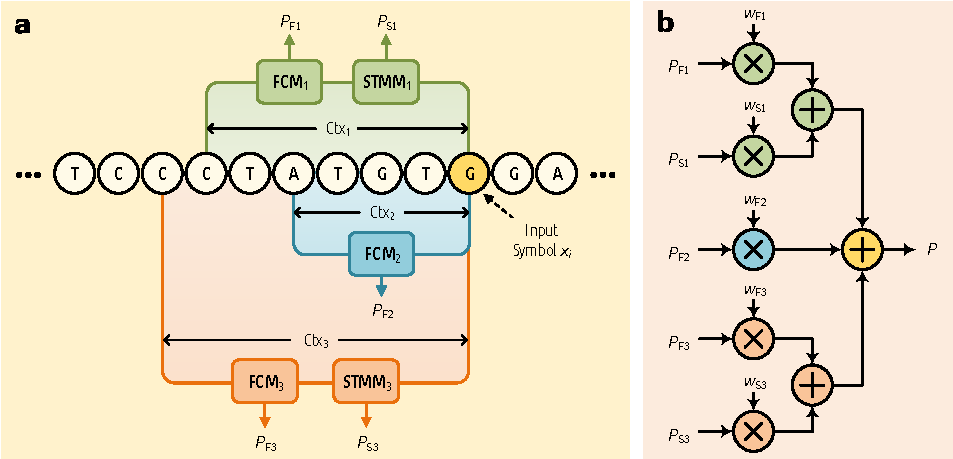
\includegraphics[width=.85\linewidth]{data_model.pdf}
\caption{model.}
\label{fig.model}
\end{figure}

\paragraph{Finite-context model (FCM)}
A finite-context model considers Markov property to estimate the probability of the next symbol in an information source, based on the past $k$ symbols (a context of size $k$)~\cite{sayood2017introduction,hosseini2019ac,pinho2013mfcompress}. Denoting the context as $c_{k,\,i} = s_{i-k} s_{i-k+1}\ldots s_{i-2} s_{i-1}$, the probability of the next symbol $s_i$ in an information source $S$, which is posed at $i$, can be estimated as
\begin{equation} \label{eq.estimate}
P_m(s_i|c_{k,\,i}) = \frac{N(s_i|c_{k,\,i})+\alpha}{N(c_{k,\,i})+ \alpha|\Theta|},
\end{equation}
in which $m$ stands for model (FCM in this case), $N(s_i|c_{k,\,i})$ shows the number of times that the information source has generated symbol~$s_i$ in the past, $|\Theta|$ denotes size of the alphabet~$\Theta$, $N(c_{k,\,i}) = \sum_{b \in \Theta} N(b|c_{k,\,i})$ represents the total number of events occurred for the context~$c_{k,\,i}$ and $\alpha$ allows to keep a balance between the maximum likelihood estimator and the uniform distribution. Eq.~\ref{eq.estimate} turns to the Laplace estimator, for $\alpha=1$, and also behaves as a maximum likelihood estimator, for large number of events~$i$~\cite{pratas2015alignment}.

\paragraph{Substitutional tolerant Markov model (STMM)}
A substitutional tolerant Markov model~\cite{pratas2017substitutional} is a probabilistic-algorithmic model that assumes at each position, the next symbol in the information source is the symbol which has had the highest probability of occurrence in the past. This way, an STMM ignores the real next symbol in the source. Denoting the past $k$ symbols as $c_{k,\,i} = s_{i-k} s_{i-k+1}\ldots s_{i-2} s_{i-1}$, the probability of the next symbol $s_i$, can be estimated as
\begin{equation}
P_m(s_i|{c'}_{k,\,i}) = \frac{N(s_i|{c'}_{k,\,i})+\alpha}{N({c'}_{k,\,i})+ \alpha|\Theta|},
\end{equation}
where $N$ represents the number of occurrences of symbols, that is saved in memory, and ${c'}_{k,\,i}$ is a copy of the context $c_{k,\,i}$ which is modified as 
\begin{equation}
{c'}_{k,\,i} = \argmax_{\forall b\in \Theta}{P_m(b|{c'}_{k,\,i})}.
\end{equation}

STMMs can be used along with FCMs to modify the behavior of \smashpp in confronting with nucleotide substitutions in genomic sequences. These models have the potential to be disabled, to reduce the number of mathematical calculations and consequently, increase the performance of the proposed method. Such operation is automatically performed using an array of size $k$ (the context size), named history, which preserves the past $k$ hits/misses. Seeing a symbol in the information source, the memory is checked for the symbol with the highest number of occurrences. If they are equal, a hit is saved in the history array; otherwise, a miss is inserted into the array. Before getting to store a hit/miss in the array, it is checked for the number of misses and in the case they are more than a predefined threshold $t$, the STMM will be disabled and also the history array will be reset. This process is performed for each symbol in the sequence.

This example shows the distinction between a finite-context model and a substitutional tolerant Markov model. Assume, the current context at position $i$ is $c_{11,\,i}=\textrm{GGCTAACGTAC}$, and the number of occurrences of symbols saved in memory is $\textrm{A}=10$, $\textrm{C}=12$, $\textrm{G}=13$ and $\textrm{T}=11$. Also, the symbol to appear in the sequence is $\textrm{T}$. An FCM would consider the next context as $c_{11,\,i+1}=\textrm{GCTAACGTACT}$, while an STMM would consider it as ${c'}_{11,\,i+1}=\textrm{GCTAACGTACG}$, since the base $\textrm{G}$ is the most probable symbol, based on the number of occurrences stored in memory.

\paragraph{Cooperation of FCMs and STMMs}
When FCMs and STMMs are in cooperation, the probability of the next symbol $s_i$ in an information source $S$, at position $i$, can be estimated as
\begin{equation}
P(s_i) = \sum_{m\in M_F} P_m(s_i|c_{k,\,i})\;w_{m,\,i} + \sum_{m\in M_S} P_m(s_i|{c'}_{k,\,i})\;{w'}_{m,\,i}, \quad\forall s_i\in S,~1\le i\le |S|,~1\le k\le i-1
\end{equation}
in which $M_F$ and $M_S$ denote sets of FCMs and STMMs, respectively, $P_m(s_i|c_{k,\,i})$ shows the probability of the next symbol estimated by the FCM, $P_m(s_i|{c'}_{k,\,i})$ represents this probability estimated by the STMM, and $w_{m\,i}$ and ${w'}_{m,\,i}$ are weights assigned to each model based on its performance. We have
\begin{align}
\forall m\in M_F: \quad &w_{m,\,i} \propto (w_{m,\,i-1})^{\gamma_m} P_m(s_i|c_{k+1,\,i-1}),
\nonumber
\\[1mm]
\forall m\in M_S: \quad &{w'}_{m,\,i} \propto ({w'}_{m,\,i-1})^{{\gamma'}_m} P_m(s_i|{c'}_{k+1,\,i-1}),
\end{align}
where $\gamma_m$ and ${\gamma'}_m \in [0,1)$ are forgetting factors predefined for each model. Also,
\begin{equation}
\sum_{m\in M_F} w_{m,\,i} + \sum_{m\in M_S} {w'}_{m,\,i} = 1.
\end{equation}
By experimenting different forgetting factors for models, we have found that higher factors should be assigned to models that have higher context-order sizes (less complexity) and vice versa. As an example, when the context size $k=6$, $\gamma_m~\mathrm{or}~{\gamma'}_m \simeq 0.9$ and when $k=18$, $\gamma_m~\mathrm{or}~{\gamma'}_m \simeq 0.95$ would be appropriate choices. These values show that forgetting factor and complexity of a model are inversely related.

\paragraph{Storing models in memory}
The FCMs and STMMs include, in fact, count values which need to be saved in memory. For this purpose, four different data structures have been employed considering the context-order size $k$, as follows:
\begin{equation*}
  \textrm{data structure} =
\begin{cases}
  \textrm{table of 64 bit counters}, & 1 \leq k \leq 11 \\
  \textrm{table of 32 bit counters}, & k=12, 13 \\
  \textrm{table of 8 bit approximate counters}, & k=14 \\
  \textrm{Count-Min-Log sketch of 4 bit counters}. & k \ge 15
\end{cases}
\end{equation*}

\begin{figure}[!h]
  \centering
\includegraphics[height=.9\textheight]{data_struct.pdf}
\caption{data structure.}
\label{fig.struct}
\end{figure}

The table of 64 bit counters, that is shown in Fig.~\ref{fig.struct}a, simply saves number of events for each context. The table of 32 bit counters saves in each position the number of times that the associated context is observed. When a counter reaches to the maximum value $2^{32}-1=4294967295$, all the counts will be renormalized by dividing by two, as shown in Fig.~\ref{fig.struct}b.

The approximate counting is a method that employs probabilistic techniques to count large number of events, while using small amount of memory~\cite{morris1978counting}. Fig.~\ref{alg.approx} shows the algorithm for two major functions associated with this method, \textsc{Update} and \textsc{Query}. In order to update the counter, a pseudo-random number generator (PRNG) is used the number of times of the counter's current value to simulate flipping a coin. If it comes up 0/Heads each time or 1/Tails each time, the counter will be incremented. Fig.~\ref{fig.struct}c shows the difference between arithmetic and approximate counting, and also the values which are actually stored in memory. Note that since an approximate counter represents the actual count by an order of magnitude estimate, one only needs to save the exponent. For example, if the actual count is $8$, we store it in memory as $\log_2 8=3$.
\begin{figure}[b]
  \centering
  \begin{tabular}{|c|}
    \hline
\begin{minipage}[t]{.5\linewidth}
  \vspace{0pt}
  \begin{algorithmic}[1]
    % \Require table of 8 bit counters
    \Function{\textsc{IncreaseDecision}}{$x$}
    \State \textbf{return} True with probability $\frac{1}{2^x}$, else False
    \EndFunction
    \Statex
    \Function{\textsc{Update}}{$x$}
    \State $c\gets \mathrm{table}[x]$
    \If{$\textsc{IncreaseDecision($c$)}=\mathrm{True}$}
    \State $\mathrm{table}[x]\gets c+1$
    \EndIf
    \EndFunction
    \Statex
    \Function{\textsc{Query}}{$x$}
    \State $c\gets \mathrm{table}[x]$
    \State \textbf{return} $2^c-1$
    \EndFunction
  \end{algorithmic}
  \vspace{2mm}
\end{minipage}
\\ \hline
\end{tabular}
\caption{Approximate counting update and query.}
\label{alg.approx}
\end{figure}

The Count-Min-Log Sketch (CMLS) is a probabilistic data structure to save frequency of events in a table by means of a family of independent hash functions~\cite{pitel2015count}. The algorithm for updating and querying the counter is shown in Fig.~\ref{alg.cmls}. In order to update the counter, its current value is hashed with $d$ independent hash functions. Then, a coin is flipped the number of times of the counter's current value, employing a pseudo-random number generator. If it comes up 0/Heads each time or 1/Tails each time, the minimum hashed values (out of $d$ values) will be updated, as shown in Fig.~\ref{fig.struct}d.

The CMLS requires a family of pairwise independent hash functions
$H = \{h: U \to [m]\}$, in which each function $h$ maps some universe $U$ to $m$ bins. 
To have this family, we use universal hashing by randomly selecting a hash function from a universal family in which $\forall x,y\in U,~x\neq y:~~P_{h\in H}[h(x)=h(y)]\leq \frac{1}{m}$.
The hash function can be obtained by
\begin{equation}
  h_{a,b}(x)=\left((ax+b)~\bmod p\right)~\bmod m,
\end{equation}
where $p\ge m$ is a prime number and $a$ and $b$ are randomly chosen integers modulo $p$ with $a\neq 0$.

\begin{figure}[t]
  \centering
  \begin{tabular}{|c|}
    \hline
  \begin{minipage}[t]{.55\linewidth}
    \vspace{0pt}
    \begin{algorithmic}[1]
      \Require sketch width $w$, sketch depth $d$, $m$ bins, prime $p\ge m$, randomly chosen integers $a_{1..d}$ and $b_{1..d}$ modulo $p$ with $a\neq 0$
      % independent hash functions $h_{1..d}: U\to \{1..w\}$
      \Statex
      \Function{\textsc{Hash}}{$k, x$} \Comment{Universal hash family}
      \State \textbf{return} $\left((a_k x + b_k)~\bmod p\right)~\bmod m$
      \EndFunction
      \Statex
      \Function{\textsc{MinCount}}{$x$}
      \State $\mathrm{minimum}\gets 15$ \Comment{Biggest 4 bit number}
      \For{$k\gets 1\mathrm{\;to\;}d$}
      \State $h\gets \textsc{Hash}(k, x)$
      \If{$\mathrm{sketch}[k][h] < \mathrm{minimum}$}
      \State $\mathrm{minimum}\gets \mathrm{sketch}[k][h]$
      \EndIf
      \EndFor
      \State \textbf{return} $\mathrm{minimum}$
      \EndFunction
      \Statex
      \Function{\textsc{IncreaseDecision}}{$x$}
      \State \textbf{return} True with probability $\frac{1}{2^x}$, else False
      \EndFunction
      \Statex
      \Function{\textsc{Update}}{$x$}
      \State $c\gets \textsc{MinCount}(x)$
      \If{$\textsc{IncreaseDecision($c$)}=\mathrm{True}$}
      \For{$k\gets 1\mathrm{\;to\;}d$}
      \State $h\gets \textsc{Hash}(k, x)$
      \If{$\mathrm{sketch}[k][h] = c$}
      \State $\mathrm{sketch}[k][h]\gets c+1$
      \EndIf
      \EndFor
      \EndIf
      \EndFunction
      \Statex
      \Function{\textsc{Query}}{$x$}
      \State $c\gets \textsc{MinCount}(x)$
      \State \textbf{return} $2^c-1$
      \EndFunction
    \end{algorithmic}
    \vspace{2mm}
  \end{minipage}
  \\ \hline
  \end{tabular}
  \caption{Count-Min-Log Sketch update and query.}
  \label{alg.cmls}
\end{figure}

\subsection{Finding similar regions}
Our goal is to find similar regions in reference and target files.

Fig.~\ref{fig.simil}

\begin{figure}[!h]
  \centering
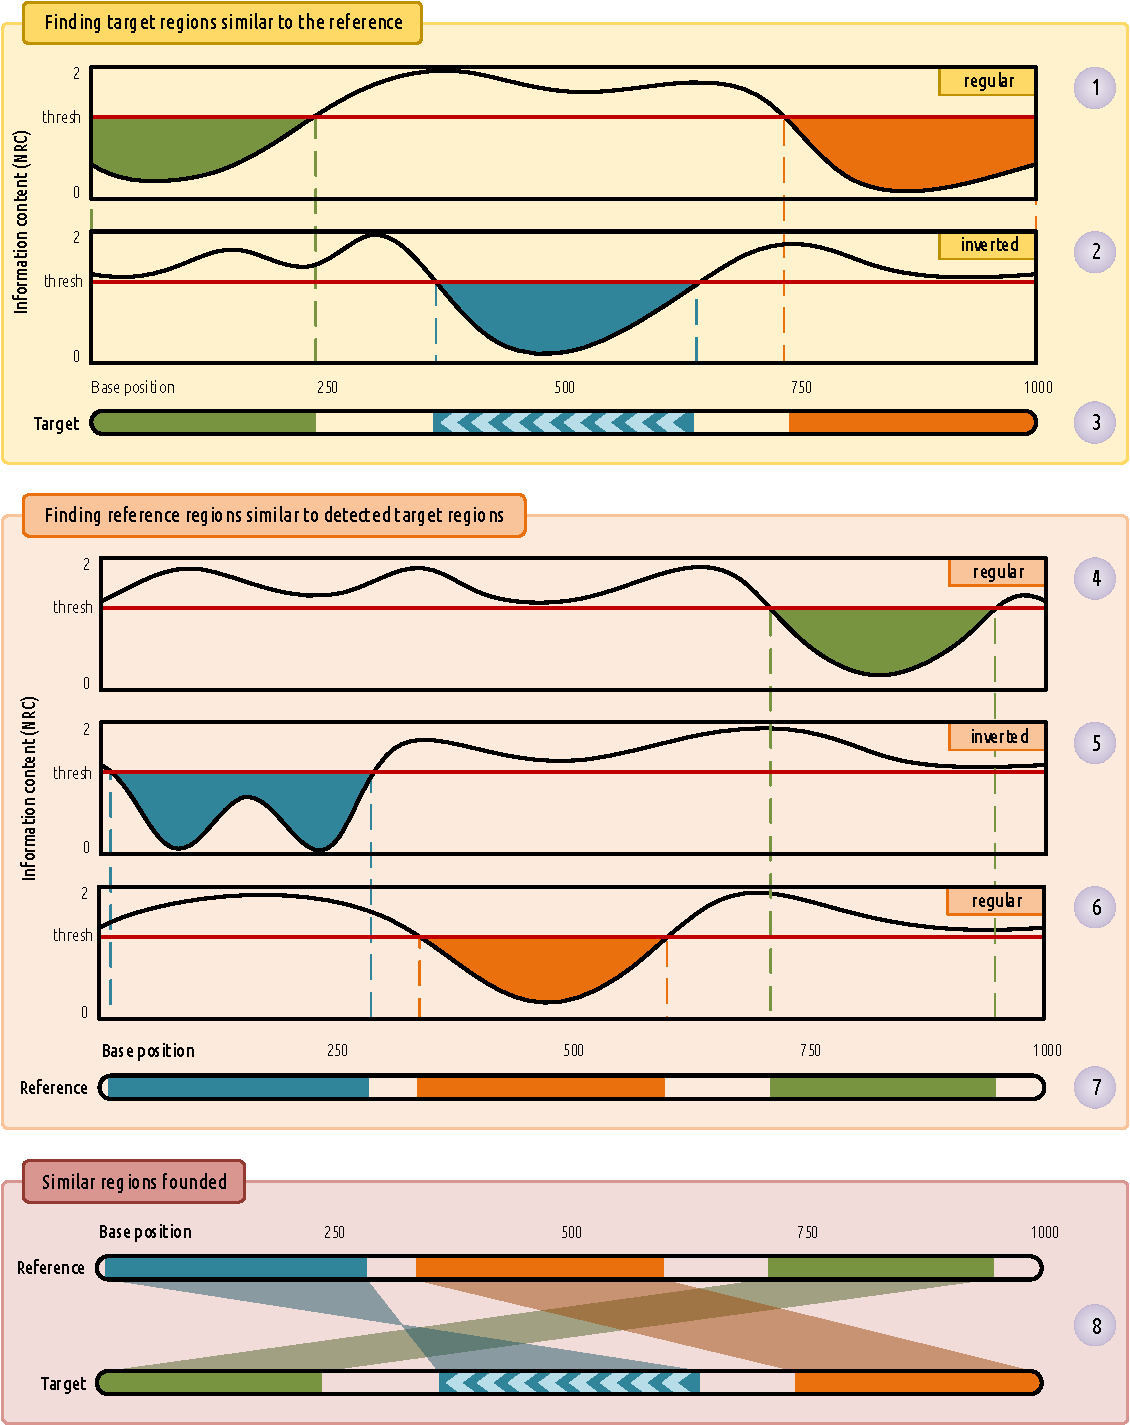
\includegraphics[width=.95\linewidth]{simil.pdf}
\caption{simil.}
\label{fig.simil}
\end{figure}

In order to smooth the profile information, we use Hann window~\cite{blackman1959particular}, which is a discrete window function given by
\begin{equation}
  \label{eq.hann}
  w[n]=0.5-0.5\;\cos \left({\frac {2\pi n}{N}}\right)=\sin ^{2}\left({\frac {\pi n}{N}}\right),
\end{equation}
where $0\le n\le N$ and length of the window is $N+1$ (Fig.~\ref{fig.hann}).

\begin{figure}[!h]
\centering
% 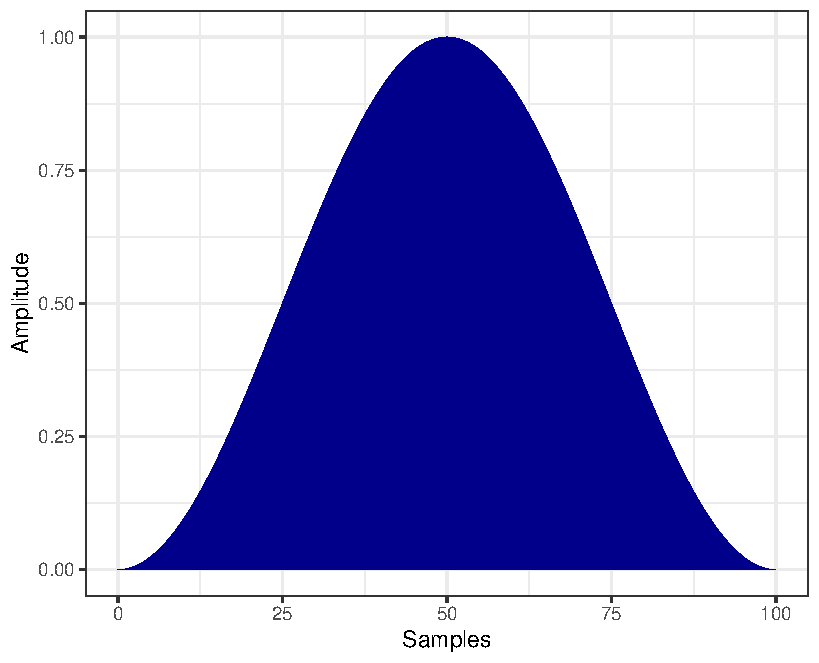
\includegraphics[width=7cm]{hann.pdf}
\caption{Hann window for 101 samples.}
\label{fig.hann}
\end{figure}

\subsection{Computing complexities}
Kolmogorov

\subsection{The software}
\label{subsec.software}

Besides Hann window that is used as default to filter the profile information obtained by the reference-based compression, we have implemented several other window functions (Fig.~\ref{fig.filters}), including Blackman~\cite{blackman1959particular}, Hamming~\cite{tukey1949measuring}, Nuttall~\cite{nuttall1981some}, rectangular~\cite{oppenheim1999discrete}, sine~\cite{harris1978use}, triangular~\cite{bartlett1950periodogram} and Welch~\cite{welch1967use} windows. These functions are given by
\begin{align}
  w[n] &= 1,
  \tag*{(rectangular)} \\
  w[n] &= 1-\left|\tfrac {n-N/2}{L/2}\right|, \quad L=N,
  \tag*{(triangular/Bartlett)} \\
  w[n] &= 1-\left(\tfrac {n-N/2}{N/2}\right)^{2},
  \tag*{(Welch)} \\
  w[n] &= \sin \left(\tfrac {\pi n}{N}\right),
  \tag*{(sine)} \\
  w[n] &= 0.54348-0.45652\;\cos \left(\tfrac {2\pi n}{N}\right),
  \tag*{(Hamming)} \\
  w[n] &= 0.42659-0.49656\;\cos \left(\tfrac {2\pi n}{N}\right)+0.07685\;\cos \left(\tfrac {4\pi n}{N}\right),
  \tag*{(Blackman)} \\
  w[n] &= 0.35577-0.48740\;\cos \left(\tfrac {2\pi n}{N}\right)+0.14423\;\cos \left(\tfrac {4\pi n}{N}\right)-0.01260\;\cos \left(\tfrac {6\pi n}{N}\right).
  \tag*{(Nuttall)} \\
\end{align}

\begin{figure}[!h]
\centering
% 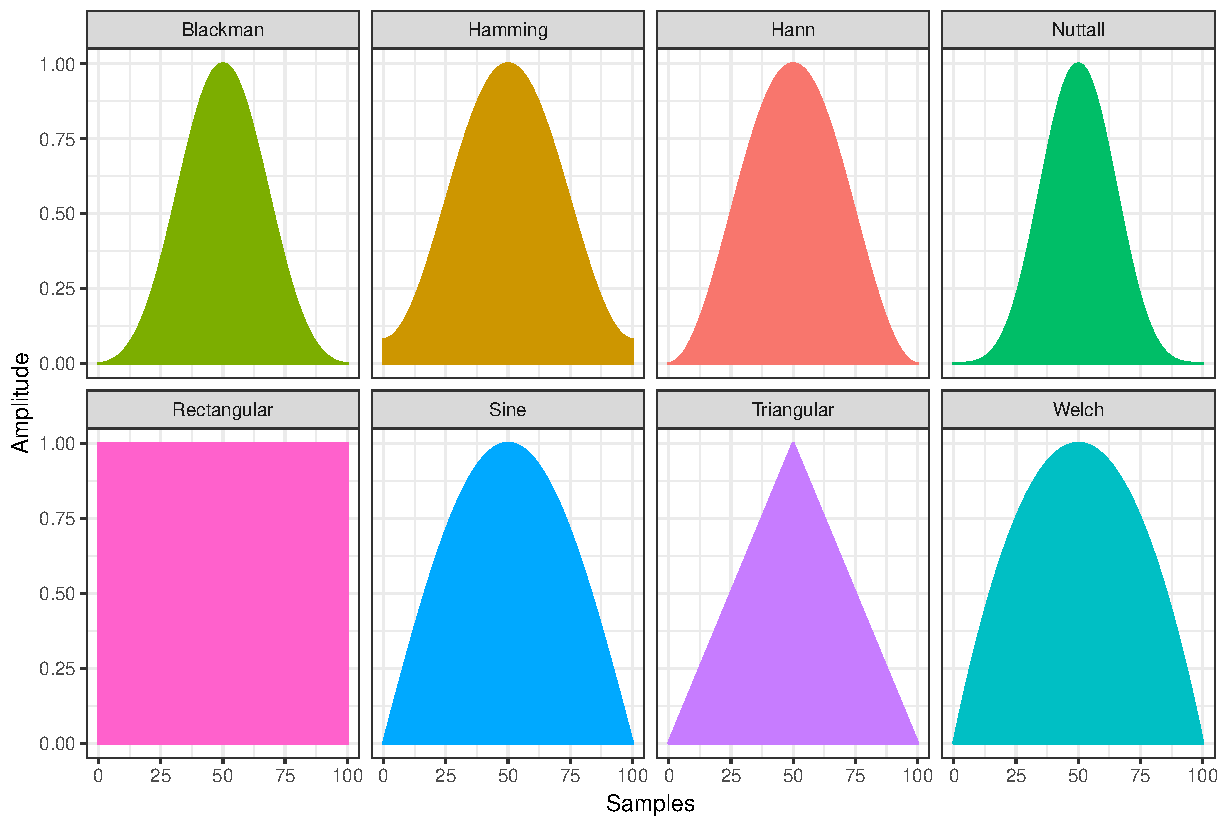
\includegraphics[width=.95\linewidth]{filters.pdf}
\caption{Window functions.}
\label{fig.filters}
\end{figure}